\documentclass{article}

\usepackage{geometry}
  \geometry{
    a4paper,
    right=25mm
  }

\usepackage{wrapfig}

\usepackage{graphicx}
\usepackage[latin1]{inputenc}
\usepackage[T1]{fontenc}
\usepackage[english]{babel}
\usepackage{listings}
\usepackage{xcolor}
\usepackage{eso-pic}
\usepackage{mathrsfs}
\usepackage{url}
\usepackage{amssymb}
\usepackage{amsmath}
\usepackage{multirow}
\usepackage{hyperref}
\usepackage{booktabs}
\usepackage{bbm}
\usepackage{cooltooltips}

\usepackage{colordef}
\usepackage{lvblisting}



\usepackage{algorithm}
\usepackage[noend]{algpseudocode}
\usepackage{ragged2e}

\makeatletter
\def\BState{\State\hskip-\ALG@thistlm}
\makeatother

\DeclareMathOperator*{\argmin}{arg\,min}

\title{Credit Default Prediction}
\author{Valeryia Mosinzova, Michail Psarakis, Thomas Siskos}
\date{ }

\begin{document}
\begin{titlepage}
  \begin{center}
  
  
\includegraphics[scale=1.25]{hulogo.pdf} \par\vspace{1cm}
  {\scshape\LARGE Humboldt University Berlin \par}
  \vspace{1cm}
  {\scshape\Large Term paper\par}
  \vspace{1.5cm}
  {\huge\bfseries Credit Default Prediction\par}
  \vspace{1cm}
  {\Large\itshape Valeryia Mosinzova, Michail Psarakis, Thomas Siskos \par}
  \vspace{1cm}
  {\Large\scshape Statistical Programming Languages\par}
  \vspace{1cm}
  \vfill
  supervised by \par
  {\Large Alla~\scshape Petukhina \par}
  \vfill
  {\large \today\par}
  \end{center}
\end{titlepage}

\tableofcontents
\newpage

\listoftables
\listoffigures
\listofalgorithms
\newpage

\section{Introduction}

The term default probability is a financial term which describes the likelihood that a borrower will fail to make scheduled repayments over a specific time horizon, which is usually a year. The effective estimation and prediction of corporate defaults are crucial for asset pricing, credit risk assessment of loan portfolios as 
well as the valuation of other financial products exposed to corporate defaults (Miao et al., 2018). This issue has been considered in several studies. There are two basic approaches to deal with default risk analysis: the market-based model (a.k.a. structural model) and the statistical approach, determined through the empirical analysis of historical data like accounting data (H{\"a}rdle et al., 2012).

In our paper we aim to perform default prediction analysis by following the methodologies of H{\"a}rdle et al. (2012), Chen et al. (2011) and Zhang \& H{\"a}rdle (2010) We seek to replicate some of their results using the \texttt{R} programming language. Our analysis is based on the creditreform-database, which provides several 
financial statement variables of German firms. In our work we perform linear and generalized linear techniques for predicting bankruptcy based on financial ratios. We compare the predictive performance between following models: logit, probit, Classification and Regression Trees (CART), Random Forests (RF) and Linear Discriminant Analysis (LDA). 

The rest of the paper is organized as follows. In the next section we describe the creditreform-dataset. In section 3 we explain the data preparation procedures as well as the variables and ratios used in this paper. Section 4 contains a brief introduction to Binary Response Models, with a custom implementation and an application of a Logit model to the creditreform-dataset. In section 5 we apply Classification and Regression Trees (CART), which is followed by a section about Random Forests (RF). Linear Discriminant Analysis (LDA) is briefly explained and applied in section 6. In Section 7, we present the steps we take to evaluate predictions of the selected models and the suitable performance measures. Finally section 8 summarises the conclusions we draw from our analysis.

\section{The dataset}

We used the creditreform database obtained from the Laboratory for Empirical and Quantitative Research (LEQR) of the Humboldt University of Berlin \href{https://leqr.wiwi.hu-berlin.de/leqr/content/databaseInformation/creditreform/creditreform.htm}{(leqr.wiwi.hu-berlin.de)} to analyse a sample of 20,000 solvent and 1,000 insolvent German firms from the period of 1996-2007. Due to incomplete data from 2003 onwards and missing data for insolvent firms in 1996 we will focus our analysis on the data of the period between 1997 and 2002. About half of the data refers to the years 2001 and 2002. The majority of firms appear several times in different years in the dataset, while the data for the insolvent firms was collected two years prior to the default (Chen et al. (2011)). Each firm is described by several financial statement variables as those in balance sheets and income statements. A complete list of all variables of the creditreform database as well as their descriptions is provided in table \ref{creditVars}. 

The firms are divided into the sectors of construction (39.7\%), manufacturing (25.7\%), wholesale and retail trade (20.1\%), real estate (9.4\%) and others (5.1\%). The respective composition of solvent firms is manufacturing (27.4\%), wholesale and retail trade(24.8\%), real estate (16.9\%), construction (13.9\%) and others (17.1\%), including publishing, administration and defence, education and health (Chen et al. 2011). In our project we focus on the four largest industry sectors.

\begin{center}
\begin{table}
\centering
\caption{Variables of the Creditreform database}
\label{creditVars}
\begin{tabular}{cc} 
\hline\hline
Column & Value\\
\hline
ID & ID of each company\\
T2 & Solvency status (solvent:0, insolvent:1)\\
Jahr & Year\\
VAR1 & Cash and cash equivalents\\
VAR2 & Inventories\\
VAR3 & Current assets\\
VAR4 & Tangible assets\\
VAR5 & Intangible assets\\
VAR6 & Total assets\\
VAR7 & Accounts receivable\\
VAR29 & Accounts receivable vs. affiliated companies\\
VAR8 & Lands and buildings\\
VAR9 & Equity (own funds)\\
VAR10 & Shareholder loan\\
VAR11 & Accrual for pension liabilities\\
VAR12 & Total current liabilities\\
VAR13 & Total longterm liabilities\\
VAR14 & Bank debt\\
VAR15 & Accounts payable\\
VAR30 & Accounts payable vs. affiliated companies\\
VAR16 & Sales\\
VAR17 & Administrative expenses\\
VAR18 & Amortization and depreciation\\
VAR19 & Interest expenses\\
VAR20 & Earnings before interest and taxes (EBIT)\\
VAR21 & Operating income\\
VAR22 & Net income\\
VAR23 & Increase (decrease) in inventories\\
VAR24 & Increase (decrease) in liabilities\\
VAR25 & Increase (decrease) in cash\\
VAR26 & Industry classification code\\
VAR27 & Legal form\\
VAR28 & Number of employees\\
Rechtskreis & Accounting principle\\
Abschlussart & Type of account\\
\hline\hline
\end{tabular}
\end{table}
\end{center}

\section{Data preparation}

For cleaning the data we use primarily the \texttt{dplyr} package, which allows us to manipulate data easier than with base \texttt{R} allowing for less verbose, i.e. more easily readable code. In order to clean the data we load the Creditreform dataset into \texttt{R} with the \texttt{read.csv()} command and store it as \texttt{data}. Using \texttt{dplyrs}'s \texttt{filter()} command we choose only those observations from the years between 1997-2002 and store them as \texttt{data1}.

\lstinputlisting[language=R, firstline=4, lastline=10, firstnumber=4, escapechar=|, caption={|\textbf{\href{https://github.com/thsis/SPL_WS1718/blob/master/Preparation/data.preparation.R}{data.preparation.R}}|}]{../Preparation/data.preparation.R}

We then want to choose only those observations belonging to the four most prevalent industry sectors in both solvent and insolvent firms, i.e manufacturing, wholesale and retail trade, real estate and construction. We extract the industry class of firms by using the \texttt{substring()} command and save it in a new column of \texttt{data1}.

\lstinputlisting[firstline=13, lastline=13, firstnumber=13, escapechar=|, caption={|\textbf{\href{https://github.com/thsis/SPL_WS1718/blob/master/Preparation/data.preparation.R}{data.preparation.R}}|}]{../Preparation/data.preparation.R}

These two digits contained in the variable \texttt{Ind.Klasse} are then used to identify in which of the 17 broad industry sectors, defined in the German Classification of Economic Activities Edition 1993 (WZ93), issued by the German Federal Statistical Office \href{https://www.destatis.de/DE/Methoden/Klassifikationen/GueterWirtschaftklassifikationen/Content75/KlassifikationWZ93.html}{(destatis.de)}, each firm belongs. If the value of the variable is in the range 15-37 then the firm belongs to the manufacturing sector. Accordingly the ranges 50-52 and 70-74 correspond to "Wholesale and Retail Trade" and "Real Estate" respectively, while the value 45 corresponds to "Construction". We create four subsets of data1 for each of the above mentioned sectors by using the \texttt{filter()} command again and remove \texttt{data} and \texttt{data1} with the \texttt{rm()} command as we do not need them anymore. The 4 subsets are then bound with \texttt{rbind()} into a new dataset with the name \texttt{data}. 

\lstinputlisting[language=R, firstline=22, lastline=39, firstnumber=22, escapechar=|, caption={|\textbf{\href{https://github.com/thsis/SPL_WS1718/blob/master/Preparation/data.preparation.R}{data.preparation.R}}|}]{../Preparation/data.preparation.R}

We then turn our interest on the size of the companies. Specifically the distribution of total assets which can be considered to be representative of the distribution of the companies' size (Chen et al., 2011). Following the methodology of Zhang \& H{\"a}rdle (2010), we keep only firms with total assets (\texttt{VAR6} in the dataset) in the range of $10^5 - 10^8$ Euros, since the credit quality of small firms often depends mostly on the finances of a key individual (e.g. the owner).

Finally, we eliminate observations with zero values in variables used as denominators in the calculation of the financial ratios that will be used for the classification of the companies (lines 60-67 in the code) and save the result as \texttt{data\_clean}. 

\lstinputlisting[language=R, firstline=60, lastline=67, firstnumber=60, escapechar=|, caption={|\textbf{\href{https://github.com/thsis/SPL_WS1718/blob/master/Preparation/data.preparation.R}{data.preparation.R}}|}]{../Preparation/data.preparation.R}

We end up with 9591 solvent and 783 insolvent firms, which is a similar result as in Chen et al. (2010). 

\begin{table}
\caption{Number of solvent and insolvent companies per year in the dataset}
\label{finRatios}
\begin{center}
\begin{tabular}{ccc} 
\hline\hline
Year & Solvent & Insolvent\\ 
\hline
1997 & 1084 & 126 \\
1998 & 1175 & 114 \\
1999 & 1277 & 147 \\
2000 & 1592 & 135 \\
2001 & 1920 & 132 \\
2002 & 2543 & 129 \\
\hline\hline
\end{tabular}
\end{center}
\end{table}

\subsection{Financial Ratios}

The Creditreform database contains many financial statement variables for each company. Such statements are often used by investors to evaluate firms in two basic ways. A firm is either compared with itself by analysing how it has changed over time, or the firm is compared to other similar firms by means of a common set of financial ratios (Berk \& DeMarzo, 2016).  We follow the methodology of Chen et al. (2011) and use 23 financial statement variables to create 28 financial ratios to be used in classification. The variables used in the creation of the financial ratios are summarized in table \ref{finRatios}. These financial ratios can be divided into six main groups (risk factors): profitability, leverage, liquidity, activity, firm size and percentage change for some variables.

Table \ref{finRatios} presents all the financial ratios used in the current study, the formulas used for their calculation and their category. In our code, the calculation procedure of the financial ratios can be found in lines 92-121 where we add the ratios for each firm to the dataset by using the \texttt{dplyr}'s \texttt{mutate()}-command. Then we create a dataset \texttt{test\_data\_rel} where only relevant variables are kept, i.e. the ID of the firm, it's solvency status, the year as well as the 28 financial ratios. 

\begin{table}
\begin{center}
\caption{Variables used for the calculation of financial ratios and their description}
\footnotesize
\begin{tabular}{cccc} 
\hline\hline
Variable  & Description & Variable & Description\\ 
\hline
VAR1 & Cash and cash equivalents & VAR14 & Bank debt\\
VAR2 & Inventories & VAR15 & Accounts payable\\
VAR3 & Current assets & VAR16 & Sales\\ 
VAR5 & Intangible assets & VAR18 & Amortization and depreciation\\
VAR6 & Total assets & VAR19 & Interest expenses\\
VAR3 - VAR2 & Quick assets & VAR20 & EBIT\\
VAR7 & Accounts receivable & VAR21 & Operating income\\
VAR8 & Lands and buildings & VAR22 & Net income\\
VAR9 & Equity (own funds) & VAR23 & Increase (decrease) inventories\\
VAR12 & Total current liabilities & VAR24 & Increase (decrease) liabilities\\
VAR12 + VAR13 & Total liabilities & VAR25 & Increase (decrease) cash\\
VAR3 - VAR12 & Working capital & &\\ 
\hline\hline
\end{tabular}
\end{center}
\end{table}

Profitability ratios have appeared in many studies to be strong predictors for bankruptcy (Chen et al., 2011). They measure the ability of a firm to generate revenue relative to its costs over a specific time period. We calculate 7 ratios belonging to this group (ratios x1-x7). The return on assets ratio (x1), for example, provides information on how effective a firm is in making use of its assets to create income. A higher ratio signals that a firm is able to earn more money on less investment (Chen et al., 2011). 

Among the profitability ratios, the net profit margin ratio \texttt{x2} shows the percentage of sales which the firm keeps in earnings. A high ratio corresponds to a firm with more profitability and better control over its costs (Chen et al., 2011).  

\lstinputlisting[language=R, firstline=92, lastline=121, firstnumber=92, escapechar=|, caption={|\textbf{\href{https://github.com/thsis/SPL_WS1718/blob/master/Preparation/data.preparation.R}{data.preparation.R}}|}]{../Preparation/data.preparation.R}

Another important factor of risk measurement is leverage. It refers to the extent that a firm relies on debt as a source of financing (Berk \& DeMarzo, 2016). As firms combine debt and equity to finance their operations, leverage ratios are useful in evaluating a firm's ability to meet its financial obligations. We calculate 7 ratios belonging to this group (\texttt{x8-x14}). An example of a leverage ratio is the net indebtedness \texttt{x11} which measures the level of short term liabilities not covered by the firm's most liquid assets as a proportion to the firm's total assets. Except from measuring the short term leverage of a firm, this ratio provides a measure of liquidity as well. Another popular leverage ratio is the debt ratio \texttt{x13}, which is defined as the debt of a company divided by its total assets. While this ratio performs well for public firms, it performs  considerably worse for private firms compared to the total liabilities to total assets ratio \texttt{x12}. The reason for that is that liabilities is a more inclusive term which includes debt, deferred taxes, minority interest, accounts payable and other liabilities (Chen et al.,2011).
 
 The next six financial ratios we calculate belong to the family of liquidity ratios (\texttt{x15-x20}). Liquidity is a common variable in many credit decisions and represents a firm's ability to convert an asset into cash quickly (Chen et al.,2011). Liquidity ratios are important indicators of a firm's health as they assess its ability to meet its debt obligations. Chen et al. (2011) note that the cash to total assets ratio \texttt{x15} is the most important single variable relative to default in the private dataset. The quick ratio \texttt{x17} is an indicator used to assess if a firm has adequate liquidity to meet short term needs. A higher quick ratio indicates that a cash shortfall of the firm is less likely to occur in the near future (Berk \& DeMarzo, 2016). 
 
 Another type of ratios which deliver important information on insolvency are the activity ratios \texttt{x21-x24}. They measure the efficiency of a firm in using its own resources to generate cash and revenue. The asset turnover ratio \texttt{x21} measures the ability of a company to produce sales from its assets by comparing sales to its asset base. Accounts receivable \texttt{x23} and accounts payable \texttt{x24} turnover ratios are powerful predictors (Chen et al., 2011).  

\begin{table}[t]
\begin{center}
\caption{Definitions of financial ratios}
\scriptsize
\begin{tabular}{cccc} 
\hline\hline
Ratio No. & Formula & Ratio & Category\\ 
\hline
x1 & VAR22/VAR6 & Return on assets (ROA) & Profitability\\
x2 & VAR22/VAR16 & Net profit margin & Profitability\\
x3 & VAR21/VAR6 & & Profitability\\
x4 & VAR21/VAR16 & Operating profit margin & Profitability\\
x5 & VAR20/VAR6 & & Profitability\\
x6 & (VAR20+VAR18)/VAR6 & EBITDA & Profitability\\ 
x7 & VAR20/VAR16 & & Profitability\\
x8 & VAR9/VAR6 & Own funds ratio (simple) & Leverage\\
x9 & (VAR9-VAR5)/(VAR6-VAR5-VAR1-VAR8) & Own funds ratio (adjusted) & Leverage\\
x10 & VAR12/VAR6 & & Leverage\\
x11 & (VAR12-VAR1)/VAR6 & Net indebtedness & Leverage\\
x12 & (VAR12+VAR13)/VAR6 & & Leverage\\
x13 & VAR14/VAR6 & Debt ratio & Leverage\\
x14 & VAR20/VAR19 & Interest coverage ratio & Leverage\\  
x15 & VAR1/VAR6 & & Liquidity\\
x16 & VAR1/VAR12 & Cash ratio & Liquidity\\
x17 & (VAR3-VAR2)/VAR12 & Quick ratio & Liquidity\\
x18 & VAR3/VAR12 & Current ratio & Liquidity\\ 
x19 & (VAR3-VAR12)/VAR6 & & Liquidity\\
x20 & VAR12/(VAR12+VAR13) & & Liquidity\\
x21 & VAR6/VAR16 & Asset turnover & Activity\\
x22 & VAR2/VAR16 & Inventory turnover & Activity\\
x23 & VAR7/VAR16 & Accounts receivable turnover & Activity\\
x24 & VAR15/VAR16 & Accounts payable turnover & Activity\\
x25 & log(VAR6) & & Size\\
x26 & VAR23/VAR2 & Percentage of incremental inventories & Percentage\\
x27 & VAR24/(VAR12+VAR13) & Percentage of incremental liabilities & Percentage\\
x28 & VAR25/VAR1 & Percentage of incremental cash flow & Percentage\\ 
\hline\hline
\end{tabular}
\end{center}
\end{table}

 Additionally, we compute a risk indicator accorting to the size of each firm, which is defined as the logarithm of total assets \texttt{x25} in order to study the insolvency risk of small, medium and large firms (Chen et al., 2011). Finally, we calculate the ratios of the percentage change of incremental inventories, liabilities and cash flow (\texttt{x26-x28}). As the increased cash flow is the additional operating cash flow that an entity receives from taking on a new project, a positive incremental cash flow means that the firm's cash flow will increase with the acceptance of a project, the ratio of which indicates that the firm should invest time and money in the project (Chen et al., 2011). 

\lstinputlisting[language=R, firstline=80, lastline=88, firstnumber=80, escapechar=|, caption={|\textbf{\href{https://github.com/thsis/SPL_WS1718/blob/master/Preparation/data.preparation.R}{data.preparation.R}}|}]{../Preparation/data.preparation.R}

\begin{table}[t]
\begin{center}
\label{finantialRatios}
\caption{Three number summary of the financial ratios for solvent and insolvent firms.}
\footnotesize
\begin{tabular}{c|ccc|ccc} 
\hline\hline
&&Insolvent&&&Solvent&\\ 
\hline
Ratio & $q_{0.05}$ & Median & $q_{0.95}$ & $q_{0.05}$ & Median & $q_{0.95}$\\
\hline
x1 & -0.19 & 0.00 & 0.09 & -0.09 & 0.02 & 0.19\\
x2 & -0.15 & 0.00 & 0.06 & -0.07 & 0.01 & 0.09\\
x3 & -0.22 & 0.00 & 0.10 & -0.11 & 0.03 & 0.27\\
x4 & -0.16 & 0.00 & 0.06 & -0.08 & 0.02 & 0.13\\
x5 & -0.09 & 0.02 & 0.13 & -0.09 & 0.05 & 0.27\\
x6 & -0.13 & 0.07 & 0.21 & -0.04 & 0.11 & 0.35\\
x7 & -0.14 & 0.01 & 0.10 & -0.07 & 0.02 & 0.14\\
x8 & 0.00 & 0.05 & 0.40 & 0.00 & 0.14 & 0.60\\
x9 & -0.01 & 0.05 & 0.56 & 0.00 & 0.16 & 0.96\\
x10 & 0.18 & 0.52 & 0.91 & 0.09 & 0.42 & 0.88\\
x11 & 0.12 & 0.49 & 0.89 & -0.05 & 0.36 & 0.83\\
x12 & 0.29 & 0.76 & 0.98 & 0.16 & 0.65 & 0.96\\
x13 & 0.00 & 0.21 & 0.61 & 0.00 & 0.15 & 0.59\\
x14 & -7.75 & 1.05 & 7.19 & -6.76 & 2.16 & 74.37\\
x15 & 0.00 & 0.02 & 0.16 & 0.00 & 0.03 & 0.32\\
x16 & 0.00 & 0.03 & 0.43 & 0.00 & 0.08 & 1.41\\
x17 & 0.18 & 0.68 & 1.88 & 0.24 & 0.94 & 4.55\\
x18 & 0.57 & 1.26 & 3.72 & 0.64 & 1.58 & 7.15\\
x19 & -0.32 & 0.15 & 0.63 & -0.22 & 0.25 & 0.73\\
x20 & 0.34 & 0.84 & 1.00 & 0.22 & 0.86 & 1.00\\
x21 & 0.24 & 0.61 & 2.31 & 0.16 & 0.48 & 2.01\\
x22 & 0.02 & 0.16 & 0.88 & 0.01 & 0.11 & 0.56\\
x23 & 0.02 & 0.12 & 0.33 & 0.00 & 0.09 & 0.25\\
x24 & 0.03 & 0.14 & 0.36 & 0.01 & 0.07 & 0.23\\
x25 & 13.01 & 14.87 & 17.16 & 12.82 & 15.41 & 17.95\\
x26 & -1.20 & 0.00 & 0.74 & -0.81 & 0.00 & 0.57\\
x27 & -0.44 & 0.00 & 0.47 & -0.53 & 0.00 & 0.94\\
x28 & -12.17 & 0.00 & 0.94 & -7.03 & 0.00 & 0.91\\
\hline\hline
\end{tabular}
\end{center}
\end{table}
 
 In order to avoid sensitivity to outliers in applying the Random Forest, CART and the logit model, we follow the methodogy of Chen et al. (2011) and we replace extreme ratio values according to the following rule: For i = 1, ..., 28, if $x_i<q_{0.05}(x_i)$, then $x_i=q_{0.05}(x_i)$, and if $x_i>q_{0.95}(x_i)$, then $x_i=q_{0.95}(x_i)$, where $q_{0.05}(x_i)$ and $q_{0.95}(x_i)$ refer to the 0.05 and 0.95 quantiles of the ratio $x_i$ respectively. This will make our results robust and insensitive to outliers. For that purpose we create the function \texttt{replace\_extreme\_values()} (lines 80-88), which is then separately applied to the subsets of solvent and insolvent companies. The lower and upper quantile as well as the median of the financial ratios for solvent and insolvent firms are presented in table \ref{finantialRatios}. The final clean dataset to be used in further analysis is then created by binding the two subsets of solvent and insolvent firms and is saved as \texttt{data\_clean}. The resulting dataframe coincides almost entirely with the results reported by Chen et al. (2011).


\section{Linear Discriminant Analysis}
\subsection{Theory}

Since we are mostly interested in classifying if a company is going to default or not, we opted for a method that is especially suited to separate labelled data. Linear Discriminant Analysis (LDA) is a technique for dimensionality reduction that encorporates information on class-labels of the different observations. In contrast to  Principal Component Analysis, which is a unsupervised dimensionality reduction technique, it finds the rotation that ensures the highest separability between classes. It accomplishes this goal by trying to maximize between class variance while simultaneously minimizing the within class variance (H{\"a}rdle, 2003).

\begin{equation}
max\ J_{b}(w) = w \prime S_{b} w, \qquad w \in \mathbb{R}^d, d \in \mathbb{N}
\end{equation}

\begin{equation}
min\ J_{w}(w) = w \prime S_{w} w
\end{equation}

This is done by maximizing the so called Rayleigh coefficient
\begin{equation}
\label{LDA}
max J = \frac{J_b(w)}{J_w(w)} = \frac{w \prime S_{b} w}{w \prime S_{w} w}.
\end{equation}

The matrices for between and within class variance are defined as
\begin{equation}
S_b = \sum_{c=1}^{C}(\mu_c - \mu)(\mu_c - \mu)\prime
\end{equation}

\begin{equation}
\label{Sw}
S_w = \sum_{c=1}^{C}\sum_{i \in c}(x_i - \mu_c)(x_i - \mu_c)\prime
\end{equation} 

where $C$ is the number of classes, $\mu_c$ is the vector of sample means for each class respectively and $\mu$ is the vector of sample means for the full dataset. For identification purposes we can always chose weights $w$ such that $w\prime S_w w = 1$, since $J$ is constant with regards to rescalings. We can therefore replace $w$ by $\alpha w$ which will result in the constant $\alpha$ canceling out. This way the initial optimization problem can be formulated as

\begin{equation}
\argmin_{w} -\frac{1}{2} w\prime S_b w \quad s.t. \quad w \prime S_w w = 1
\end{equation}

with the lagrangian being

\begin{equation}
\mathcal{L} = -\frac{1}{2} w\prime S_b w + \frac{1}{2}\lambda\left(w\prime S_w w - 1\right).
\end{equation}

The halves are added for more convenient matrix derivatives. The Karush-Kuhn-Tucker conditions imply that the solution to this maximization problem and subsequently the vector of weights we want to find needs to fulfill

\begin{equation}
\label{LDAsolution}
S_b w = \lambda S_w w.
\end{equation}

Which results in a generalized eigenvalue problem (Duda, 1973). For solving these, there exists a convenient \texttt{R}-solution in the form of the \texttt{geigen}-package.

\subsection{Implementation}

The result from \ref{LDAsolution}, which is essentially the rotation of the underlying data's column space that ensures the highest separability, is implemented in the \texttt{lda}-class for the two-class case. The \texttt{lda()} function accepts two arguments:

\begin{enumerate}
\item \texttt{data}: a \texttt{data.frame} containing at least one column of factors indicating the class label.
\item \texttt{by}: a \texttt{character}-string equal to the column's name containing the class labels. Note that all other non-numerical columns will be ignored by the function, since LDA is only meaningful for continuous variables.
\end{enumerate} 

The function in a first step extracts the useable columns and the number of classes provided in \texttt{data}. It then performs a quick check if the prerequisites are met and then continues with the calculation of the class-means $\mu_1$ and $mu_2$, the overall mean $\mu$, as well as the scatter-matrices $S_b$ and $S_w$. With these we can solve the generalized eigenvalue problem from \ref{LDAsolution}.

\begin{algorithm}
\caption{\texttt{lda()}} \label{lda-function}
\begin{algorithmic}[1]
\Procedure{Set up Auxiliary Variables}{}
\State $\textit{num} \gets \textbf{extract numeric columns}$
\State $\textit{classes} \gets \textbf{extract class labels}$
\State $\textit{mu} \gets \textbf{calculate class means}$
\State $\textit{x\_bar} \gets \textbf{calculate overall means}$
\State $\textit{S} \gets \textbf{calculate variance per group}$
\State $\textit{S\_b1 \& S\_b2} \gets \textbf{get summands for between class scatter matrix}$
\EndProcedure

\Procedure{Calculate Scatter Matrices}{}
\State $\textit{S\_b} \gets \texttt{S\_b1 + S\_b2}$
\State $\textit{S\_w} \gets \texttt{S[[[1]] + S[[2]]}$
\EndProcedure

\Procedure{Solve Generalized Eigenvalue Problem}{}
\State $\textit{V} \gets \textbf{calculate Eigenvectors and Eigenvalues}$
\State $\textit{v} \gets \textbf{extract 2 Eigenvectors associated to largest Eigenvalues}$
\State $\textit{lda1 \& lda2} \gets \textbf{calculate first two LDA-Components}$
\State $\textit{inertia} \gets \textbf{calculate percentage of explained variance}$
\State $\textbf{return: } \texttt{lda1, lda2, classes, mu, v, inertia}$
\EndProcedure

\end{algorithmic}
\end{algorithm}

The first task of the \texttt{lda()}-function is to determine, if the prerequisites for further computation are met. To this avail it first asserts that the user provided a dataframe that contains at least one numeric column and a column that contains exactly two distinct class labels (lines 11-17). In a second step it calculates all required variables such as the class means $\mu_1$ and $\mu_2$, the overall mean $\mu$ and the covariance matrices for each group (lines 18-19). The class specific metrics are computed by calls to custom made functions defined in the \texttt{utils.R}-file of the \texttt{LDA}-directory. Essentially these functions are wrappers for subsetting a provided dataframe by a provided key, here this is the class-label, and and an \texttt{apply} call looping over the respective subset's columns. The \texttt{get\_class\_means()} calculates the mean inside the \texttt{apply}-function whereas \texttt{get\_class\_cov()} uses a call to the built-in \texttt{cov}-function. However note that \texttt{cov} calculates 

$$\hat{cov}(X) = \frac{1}{N-1} \sum_{i = 1}^{N}(x_i - \bar{x})(x_i - \bar{x})\prime.$$

Unfortunately this is not exactly what we want for the scatter matrix defined in \ref{Sw}. We need to multiply the resulting list of covariance matrices elementwise by the number of observations in each class minus one. We correct this before calculating the within class scatter matrix on line 31. 

\lstinputlisting[language=R, firstline=6, lastline=31, firstnumber=6, escapechar=|, caption={|\textbf{\href{https://github.com/thsis/SPL_WS1718/blob/master/LDA/lda.R}{lda.R}}|}]{../LDA/lda.R}

With the \texttt{matrix}-object \texttt{S\_w} storing the within-scatter-matrix $S_w$ and \texttt{S\_b} storing $S_b$ we can continue by solving the generalized Eigenvalue problem posed in \ref{LDAsolution}. This is done by the \texttt{geigen()} function from the \texttt{geigen} package.

\lstinputlisting[language=R, firstline=36, lastline=43, firstnumber=36, escapechar=|, caption={|\textbf{\href{https://github.com/thsis/SPL_WS1718/blob/master/LDA/lda.R}{lda.R}}|}]{../LDA/lda.R}

We extract the eigenvectors and eigenvalues from \texttt{V} (line 36) in form of a list. However, caution is required because the eigenvectors are not ordered, which is different to the implementation of eigenvalues in the \texttt{base}-function \texttt{eigen()}. Therefore we rearrange the eigenvectors according to their absolute eigenvalues (line 39). We extract only the first two eigenvectors, because we require the most informative rotations in order to produce two-dimensional plots. Additionally we compute the percentage of explained variance as 

\begin{equation}
intertia_i = \frac{\lambda_i^2}{\sum_{j=1}^{d}\lambda_{j}^{2}}.
\end{equation}

The rotations \texttt{lda1} and \texttt{lda2} are computed by an \texttt{apply}-call (lines 45-46) to an anonymous function which emulates a scalar product by multiplying the two vectors \texttt{v[, i]}, which is the $i$-th eigenvector $i \in \{1, 2\}$, with each observation in the provided dataset. Computationally this is equivalent to the matrix multiplication $Xv_i$, where $X$ is the data matrix and $v_i$ is the eigenvector.

Finally we gather the results into a \texttt{list} and sets it's class to \texttt{flda}. This allows us to augment pre-existing functions with a custom method for predicting and plotting for future objects of the\texttt{flda}-class in an object-oriented fashion.

\subsubsection{Predictions}

To make predicting with the \texttt{flda}-class as easy as plotting we augment the standard \texttt{predict} function in a similar fashion. We expect the user to have already trained an \texttt{flda}-model to which she or he wishes to apply new data and obtain predictions on the class labels. 

\lstinputlisting[language=R, firstline=71, lastline=88, firstnumber=71, escapechar=|, caption={|\textbf{\href{https://github.com/thsis/SPL_WS1718/blob/master/LDA/lda.R}{lda.R}}|}]{../LDA/lda.R}

The provided new data should have a similar structure to the training data. This means that especially the order of the columns should be the same. We check for obviously non-conforming data in line 77 but we do not perform explicit tests on the order of columns. If the data has the required shape we calculate the discriminant function for each observation, which is the scalar product of the observation's data vector and the first eigenvector from the trained model. We then proceed calculating a threshold $c$ for being able to discriminate between the two groups by following the rule

\begin{equation}
c = \frac{1}{2} v \prime \left(\mu_1 + \mu_2\right) 
\end{equation}

predictions are made according to the threshold, if the value of the discriminant function is smaller than the threshold we assign the label of the first class and the second class otherwise (Duda, 1973). 

\subsubsection{Plotting}

With a trained model of the \texttt{flda}-class it may be of interest to plot the rotations in order to get a visualisable idea of the separability of the two classes. To make this as easy as possible for the end-user we implemented a \texttt{plot} method for each instance of a \texttt{flda}-class. This means that a user can simply store a call to the \texttt{lda}-function inside a variable, called \texttt{model} for example. To plot the rotations one can simply invoke \texttt{plot} on \texttt{model} as easy as with any other model class by typing \texttt{plot(model)}.

This is done by augmenting \texttt{R}'s \texttt{plot}-function using the \texttt{plot.\_\_className\_\_} syntax. Here we replace \texttt{\_\_className\_\_} by \texttt{flda}

\lstinputlisting[language=R, firstline=61, lastline=69, firstnumber=61, escapechar=|, caption={|\textbf{\href{https://github.com/thsis/SPL_WS1718/blob/master/LDA/lda.R}{lda.R}}|}]{../LDA/lda.R}

We overwrite the behavior of \texttt{plot} in order to accomodate \texttt{flda}-objects. Here we pass the model's precomputed rotations to the \texttt{ggplot2} function. The \texttt{ggplot2::\_\_function\_\_} makes it explicit that we want the \texttt{\_\_function\_\_} from the \texttt{ggplot2} package. Another benefit of this syntax is that this way we do not implicitly change a users namespace, which may potentially hide some functions by overwriting them with \texttt{ggplot2} routines and therefore may result in unexpected behavior.

Looking at the creditreform dataset we can apply our custom routines by creating a train-set first and then visualizing the results. This reveals already why LDA's predictive results are of poor quality. The feature space spanned by the financial ratios is simply not linearly separable.


\lstinputlisting[language=R, firstline=19, lastline=21, firstnumber=19, escapechar=|, caption={|\textbf{\href{https://github.com/thsis/SPL_WS1718/blob/master/LDA/creditLDA.R}{creditLDA.R}}|}]{../LDA/creditLDA.R}

\begin{figure}[b]
\caption{Using Linear Discriminant Analysis on the Creditreform Database}
\centering
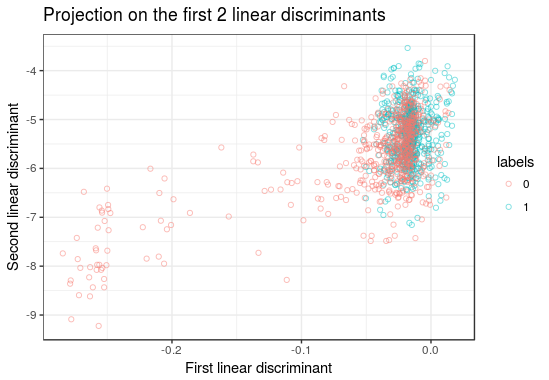
\includegraphics[scale=0.5]{../LDA/creditLDA.png}
\end{figure}

However, we can see here, that it is not possible to separate the two classes, especially by linear techniques. The plot visualises the LDA's inability to provide satisfyingly accurate predictions (H{\"a}rdle et al., 2012).


\section{Binary Response Models}
\subsection{Theory}

Logit and Probit models are the most important and probably most used member of the class of models called Binary Response or Generalized Linear Models. These parametric models are applied to estimate the probability of an observation belonging to a particular class while using observed data of known outcomes to infer models which predict the outcome of future observations.

The outcome of interest in the Creditreform-dataset is of binary nature. Firms can either go bankrupt or not. This behavior is commonly modeled by Binary Response Models like the probit or the logit model. Binary response variables follow a Bernoulli probability function

\begin{equation}
f(y|x) = P(y=1|x)^y\left(1-P(y=1|x)\right)^{1-y},\qquad y\in \{0,1\},\; x\in \mathbb{R}^d, d \in \mathbb{N},
\end{equation}

where $P(y=1|x)$ stands for the conditional probability of observing $y=1$ given $x$. Both probit and logit models have in common that $P(y=1|x)$ is modeled by a monotonic transformation of a linear function

\begin{equation}
P(y=1|x) = G(x \prime \beta), \qquad \beta \in \mathbb{R}^d,
\end{equation}

where $x \prime \beta$ is the scalar product of $x$ and $\beta$. Additionally we require that $0 \leq G(x \prime \beta) \leq 1$, since it denotes a probability.

For the probit model $G$ will be the cumulative density function of the normal distribution

\begin{equation}
P(y=1|x) = G(x \prime \beta) = \Phi(x \prime \beta) = \int_{-\inf}^{x \prime \beta} \frac{1}{\sqrt{2\pi}}exp\left[-(\frac{t^2}{2})\right]dt.
\end{equation}

Here $\Phi(x \prime \beta)$ stands for the cumulative density function of the normal distribution.

For the logit model $G$ will be replaced by the cumulative density function of the logistic distribution $\Lambda(x \prime \beta)$:

\begin{equation}
P(y=1|x) = G(x \prime \beta) = \Lambda(x \prime \beta) = \frac{exp(x \prime \beta)}{1+exp(x \prime \beta)}
\end{equation}

The parameter vector $\beta$ is obtained by the Maximum-Likelihood method. Given independent and identically distributed samples, the Likelihood function can be written as

\begin{equation}
\begin{split}
L(\beta;y, x) &= \prod_{i=1}^{n} f(y_i | x_i)
              =\prod_{i=1}^{n} P(y_i=1|x_i)^y_i\left(1-P(y_i=1|x_i)\right)^{1-y_i} \\
            & =\prod_{i=1}^{n} G(x_i\prime \beta)^y_i\left(1-G(x_i\prime \beta)\right)^{1-y_i}
\end{split}
\end{equation}

where we just take the product over all individual Bernoulli-functions.

The log-Likelihood can thus be written as
\begin{equation}
\label{logL}
l = \log L(\beta;y x) = \sum_{i=1}^{n} y_i \log G(x_i\prime \beta) +(1-y_i) \log (1-G(x_i\prime \beta))
\end{equation}

The Maximum-Likelihood estimators $\beta_ML$ are calculated as

\begin{equation}
\beta_ML = argmax(l) \\
\end{equation}

and solve the first order conditions for a maximum.

\begin{equation}
\frac{\partial l}{\partial \beta} \stackrel{!}{=} 0
\end{equation}

In general, the resulting system of equations has no closed-form solution for $\beta_ML$ and numerical solutions are needed which can be obtained by iterative optimization techniques (Winkelmann 2009). We will implement one of these methods in the next section.

\subsection{Implementation}

Our aim is to provide a function class which allows the end user to easily train a Binary Response Model of the \textit{logit} or \textit{probit} variety providing a dataset with an observed outcome variable. After training the user should also be in a position, where it is equally easy to obtain predictions for new data. With this goal in mind we created the \texttt{brm}-class. The architecture of the \texttt{brm}-class follows the general structure outlined in the chapter before. First, it generates a log-Likelihood-function, which it then optimizes using a Gradient-Descent-Algorithm. After training the model it is possible for the user to  obtain predictions by invoking the \texttt{predict()}-function, which has been augmented with a method for the \texttt{brm}-class.

\subsubsection{Obtaining the Likelihood}

The first task is to define a function that accepts a distribution and yet undefined data as it's input and first extracts all suitable variables, then expresses the Likelihood-function from \ref{logL} and finally returns another function which depends only on the weights $\beta$. This task is performed by the \texttt{get\_likehood()}-function. We outline the function pass of \texttt{get\_likehood()} first in pseudo-code followed by a look on the implementation in the \texttt{R} language.

\begin{algorithm}
\caption{get\_likehood()}\label{getllog}
\begin{algorithmic}[1]
\Procedure{Set up auxiliary variables}{}
\State $\textit{grp} \gets \text{unique labels}$
\State $\textit{nums} \gets \text{extract numeric columns}$
\State $\textit{Xy\_mat} \gets \text{bind numeric variables as a matrix}$
\State $\textit{y\_pos} \gets \text{cache position of the outcome variable}$
\EndProcedure

\Procedure{Set up log-Likelihood}{}
\State $\textit{l} \gets 0$
\State \textbf{for}: $x_i, y_i \text{in data}:$
\State \qquad $\textbf{calculate}: j = y_i \log G(x_i\prime \beta) +
               (1-y_i) \log (1-G(x_i\prime \beta)$
\State \qquad $\textbf{update}: l \gets l + j$
\State $\textbf{return}: l(\beta)$
\EndProcedure
\end{algorithmic}
\end{algorithm}

\newpage
The heavy lifting in this function is done by this \texttt{R}-snippet:
\lstinputlisting[language=R, firstline=15, lastline=25, firstnumber=15]{../BRM/logit.R}

The \texttt{for}-loop from the pseudo code is implemented as an \texttt{apply}-call to \texttt{Xy\_mat}, which in turn is a matrix of numeric columns. The \texttt{apply}-function initially selects each row in \texttt{Xy\_mat} and extracts the outcome-variable \texttt{Xy\_mat[y\_pos]} which corresponds to $y_i$ from \ref{logL}. It then computes the scalar product between the regressors of \texttt{Xy\_mat}'s row, which plays the role of $x_i \prime \beta$ in \ref{logL}. The scalar product is wrapped in \texttt{dist} which represents the cumulative distribution function $G(x\prime\beta)$ and is one of the arguments to \texttt{get\_loglikelihood()}.

\lstinputlisting[language=R, firstline=30, lastline=33, firstnumber=30, escapechar=|, caption={|\textbf{\href{https://github.com/thsis/SPL_WS1718/blob/master/BRM/logit.R}{logit.R}}|}]{../BRM/logit.R}

This way \texttt{dist} will point to the built-in functions for computing probabilities, depending if the user wishes to train a logit or a probit model. The arguments \texttt{lower.tail=TRUE} and \texttt{lower.tail=FALSE} stand for $G(x\prime \beta)$ and $G(x\prime \beta)= 1 - G(x\prime \beta))$ respectively. Finally the resulting vector is summed up and multiplied by $-1$. This is done because of the way we implemented the Gradient Descent algorithm. Currently \texttt{gradientDescentMinimizer()} can only find minima. However, Maximum-Likelihood estimation poses a maximization problem. Luckily, we can transform any maximization problem into a minimization problem by multiplying with minus one.

\subsubsection{Gradient Descent}

Since we now have a log-Likelihood function, the next step is to optimize it. To this effect we deploy a Gradient Descent algorithm. Theory tells us that in order to reach the minimum of a function $f(x)$ starting at a particular $x \in \mathbb{R}^d, d \in \mathbb{N}$ one needs to follow the negative gradient $\nabla f(x)$ of $f$ evaluated at $x$. This leads to the iterative rule we can exploit

\begin{equation}
\label{gradientDescent}
x_{t+1} = x_t - \eta \cdot \nabla f(x_t), \qquad t \in \mathbb{N}, \eta \in \mathbb{R}^+
\end{equation}

where $\eta$ is the learning rate (Duda, 1973). To this standard method of performing a Gradient Descent routine we will also make some minor modifications. First of all, we will approximate the gradients by taking finite differences, which is easier to implement albeit computationally inefficient. Finite differences are computed by

\begin{equation}
\label{finDiff}
\nabla f(x_t) \approx \frac{f(x_{t+1}) - f(x_t)}{\epsilon}, \qquad \epsilon > 0
\end{equation}

Secondly, we will before we initialize the algorithm, try a set of random points and chose the one that provides the lowest value of the objective function as a starting point for the Gradient Descent Routine. This also ensures to an extend that the algorithm, if it reaches convergence, finds the global minimum. The final modification will be to prune the gradients. When computing gradients using finite differences, it may happen that the gradient's values can become extremely high for large denominators and very small $\epsilon$. In fact, they can become high enough for \texttt{R} to treat them as \texttt{Inf} which results in the gradients being treated as \texttt{NaN} (not a number). To counteract that, we will limit the gradients to the interval $[-100, 100]$. 

\begin{algorithm}
\caption{gradientDescentMinimizer()}\label{GDM}
\begin{algorithmic}[1]
\Procedure{Set up auxiliary variables}{}
\State $\textit{learn\_rates}\gets \text{descending sequence from \texttt{learn} to 0}$
\State $\textit{a} \gets \text{matrix of 1000 randomly initialized points}$
\State $\textit{f\_a} \gets \text{vector of function values for each element of a}$
\State $\textbf{update:} a \gets \text{argmin(f\_a)}$
\State $\textit{gradient} \gets \textbf{compute gradient evaluated at a}$
\State $\textit{i} \gets 0$
\EndProcedure

\Procedure{Perform Gradient Descent}{}
\State $\textit{l} \gets 0$
\State \textbf{while}: $i \leq \textit{max\_iter} \text{ and any element of gradient} > 0:$
\State \qquad $\textbf{update}: a = a - \texttt{learn\_rates[i]} \cdot gradient$
\State \qquad $\textbf{calculate}: \textit{gradient} = \textbf{calculate gradient}$

\If {\text{i} = \text{max\_iter}} \textbf{raise} warning
\EndIf
\State $\textbf{return}: a$
\EndProcedure
\end{algorithmic}
\end{algorithm} 

The \texttt{gradientDescentMinimizer()}-function accepts following arguments:
\begin{enumerate}

\item \texttt{obj}: an objective function, that accepts exactly one argument called 'x'.
\item \texttt{n\_pars}: an integer specifying the dimensions of the objective.
\item \texttt{epsilon\_step}: a float defining the stepwidth used for computing the finite differences.
\item \texttt{max\_iter}: an integer for the maximum number of iteration before the algorithm aborts.
\item \texttt{precision}: a float defining the precision of the solution. All elements of the gradient have to be absolutely lower than \texttt{precision} for the algorithm to converge.
\item \texttt{learn}: a positive float representing the learning rate.
\item \texttt{verbose}: a boolean indicating if additional information during training is desired. The default is \texttt{FALSE}
\item \texttt{report\_freq}: If \texttt{verbose} is \texttt{TRUE}, define how often to print the logstring. The default is 10 which corresponds to a console output being printed every 10 steps.

\end{enumerate}

\lstinputlisting[language=R, firstline=143, lastline=148, firstnumber=143, escapechar=|, caption={|\textbf{\href{https://github.com/thsis/SPL_WS1718/blob/master/BRM/utils.R}{utils.R}}|}]{../BRM/utils.R}

We begin by filling the matrix \texttt{a} with 1000 \texttt{n\_pars}-dimensional points which we draw from the uniform distribution, making use of \texttt{R}'s built-in \texttt{runif}-function. We draw random numbers within the range of $[-100, 100]$ to cover a wide part of the objective function's domain.  

\lstinputlisting[language=R, firstline=130, lastline=139, firstnumber=130, escapechar=|, caption={|\textbf{\href{https://github.com/thsis/SPL_WS1718/blob/master/BRM/utils.R}{utils.R}}|}]{../BRM/utils.R}

The workhorse in this routine is the \texttt{get\_gradient()}-function, which computes the finite differences. First we need to compute the values of the objective function at the current and next step (lines 146 and 147). Then we can apply the current and next step as inputs to the objective function and compute the difference $f(x_{t+1}) - f(x_t)$. The current step is provided as the \texttt{x} argument to the function call. The next steps need to be inferred by the function. If $f(x_t)$ is multidimensional we need to perform an $\epsilon$-step in each dimension of the vector, since we want to approximate the partial derivatives of $f(x)$ evaluated at $x_t$. I.e. first we want to increment just the first element of $x$ and store the result, then just the second element, and repeat the process until we reach the last element. If we stack these vectors, we get a matrix of one-directional $\epsilon$-steps that are essentially updates of the starting point $x_t$. The objective function is then evaluated at these updated points. The gradients are then computed as the element-wise difference of the updated point compared with the start, normalized by \texttt{epsilon\_step}. The gradients are finally trimmed if necessary and returned.

\begin{algorithm}
\caption{get\_gradient()}\label{getGrad}
\begin{algorithmic}[1]
\Procedure{Set up auxiliary variables}{}
\State $$\textit{init} \gets \begin{bmatrix}
x_1 & x_2 & \cdots\\
x_1 & x_2 & \cdots\\
x_1 & x_2 & \cdots\\
\vdots & \ddots & \cdots
\end{bmatrix} $$

\State $$\textit{steps} \gets 
\begin{bmatrix}
x_1 + \epsilon & x_2 & \cdots\\
x_1 & x_2 + \epsilon & \cdots\\
x_1 & x_2 & \cdots\\
\vdots & \ddots & \cdots
\end{bmatrix}$$

\State $\textit{f\_comp} \gets \textbf{apply row-wise:} \text{ objective function to } \textit{init}$
\State $\textit{f\_steps} \gets \textbf{apply row-wise:} \text{ objective function to } \textit{steps}$
\EndProcedure

\Procedure{Compute finite differences}{}
\State $$\textit{D} \gets \frac{f\_steps - f\_comp}{\epsilon}$$
\If{$any d \in D \notin [-100; 100]$} \textbf{replace} \text{d by 100 $\cdot$ sign(d)}
\EndIf
\EndProcedure
\end{algorithmic}
\end{algorithm}

In each iteration the \texttt{while}-loop ensures that convergence has not been reached. This is implemented by a call to \texttt{any} wrapped around a vector of logical expressions. If any element of the gradient is still greater than the specified precision, the call to \texttt{any} will evaluate to \texttt{TRUE}. The second breaking criterion is a safeguard for the loop not to run infinitely many times. If the current iteration is larger than \texttt{max\_iter} the algorithm will break and the user will receive a warning (lines 175-176). 

\lstinputlisting[language=R, firstline=155, lastline=177, firstnumber=155, escapechar=|, caption={|\textbf{\href{https://github.com/thsis/SPL_WS1718/blob/master/BRM/utils.R}{utils.R}}|}]{../BRM/utils.R}

Should the user wish to receive information about the status of the algorithm during runtime, the optional argument \texttt{verbose} can be set to \texttt{TRUE} which will print a logstring to the console in regular intervals (lines 156-161). The results of the training are gathered together in the \texttt{out}-list. We store the calculated weights in \texttt{weights}, in \texttt{type} and \texttt{dist} we store wether a \textit{logit} or a \texttt{probit}-model was used. \texttt{dist} contains a pointer to the \texttt{R}-cumulative density functions of the correct distribution. We also store the value of the log-Likelihood-function in \texttt{likelihood\_val} for calculating test-statistics. Note however, that we did not implement this, since this paper focuses on obtaining predictions. Finally we assign the class and return \texttt{out}.

\subsubsection{Predictions}

In order to facilitate making predictions based on the \texttt{brm}-class we augmented the built-in function \texttt{predict()} with a method that works on our custom class in a predefined way.

\lstinputlisting[language=R, firstline=61, lastline=68, firstnumber=61, escapechar=|, caption={|\textbf{\href{https://github.com/thsis/SPL_WS1718/blob/master/BRM/logit.R}{logit.R}}|}]{../BRM/logit.R}

A call to \texttt{predict()} on a \texttt{brm}-model will add a column of ones to the provided \texttt{data}, to act as an intercept, and multiply the matrix with the weights calculated during training of the model (line 62). Finally these scores of the index-function $X\beta$ will be applied to the correct distribution. The distribution is stored inside \texttt{model\$distribution} which points to \texttt{pnorm} in case of \texttt{brm}-model of \texttt{mode} "probit" and a pointer to \texttt{plogis} if the \texttt{mode} is equal to "logit". 

\subsection{Using the Logit-Model on the creditreform Dataset}

We implemented a custom \textit{logit}-model but since it is using only \texttt{R}-routines it can be slow on large datasets including a high number of variables. Instead, we use the \texttt{caret} package to build a logistic regression model. This package provides a \texttt{train()} method for fitting the data being able to chose among various algorithms. We chose the algorithm by specifying the \texttt{method} parameter in order to predict the target variable (Kuhn, et al., 2017).

\lstinputlisting[language=R, firstline=42, lastline=42, firstnumber=42, escapechar=|, caption={|\textbf{\href{https://github.com/thsis/SPL_WS1718/blob/master/Logit/logit_model_fin.R}{logit\_model\_fin.R}}|}]{../Logit/logit_model_fin.R}
 
We apply the \texttt{glm} method. The function \texttt{glm()}, and the \texttt{predict} method for \texttt{glm} objects, reflect a classical approach to statistical inference. It only handles binary classification. Thus, we define our target variable \texttt{status} as categorical by using the \texttt{as.factor()} command (Stephens, 2016). All the other financial ratios are independent variables that influence the binary outcome of a target variable \texttt{status}. One important argument is \texttt{family\=binomial}. The \texttt{family()} function specifies the assumed distribution of the dependent variable \texttt{status}. In our case, we model a target variable as a binomial distribution. The binomial family accepts the links such as "logit", "probit", "cauchit", "log" and "cloglog". The \texttt{link} function links the output to a linear model. It passes the dependent variable through the link function, and then models the resulting value as a linear function of the values of independent variables. Different combinations of family functions and link functions lead to different kinds of generalized linear models (for example, Poisson, or probit). Without an explicit \texttt{link} argument, the link function defaults to standard \texttt{logit} (Zumel \& Mount, 2014). We store the resulting model in the object texttt{glm\_mod} and use \texttt{predict()} function to predict the insolvency of the German firms in the years 2000 until 2002. To this end, we pass the trained model \texttt{glm\_mod} and the test set features without the actual labels to the \texttt{predict()} function. We specify the type of prediction as \texttt{type=prob} to receive the probability for a firm's insolvency. The predicted probabilities are passed into \texttt{evaluate\_prediction} function to estimate the overall prediction power over models.

\lstinputlisting[language=R, firstline=53, lastline=53, escapechar=|, caption={|\textbf{\href{https://github.com/thsis/SPL_WS1718/blob/master/Logit/logit_model_fin.R}{logit\_model\_fin.R}}|}]{../Logit/logit_model_fin.R}

The practical advantage of logit model is that it provides insight into the impact of each predictor variable on the response variable. None of the nonparametric methods really provides this information. The coefficients of a logistic regression model can be thus treated as advice and may serve as orientation for decision making (Zumel \& Mount, 2014). Yet, the calculation and interpretation of coefficients exceeds the scope of this project. 

The logit model has some limitations. For example, if we include the wrong independent variables, the model will have little to no predictive value. It requires each data point to be independent of all other data points. If observations are related to one another, then the model will tend to overestimate the significance of those observations (Robinson, 2018). Further the method is searching for a single linear decision boundary that separates insolvent and solvent firms. This works well if the data are linearly separable. A linear separating boundary is, however, not suitable if there is doubt that the separation mechanism is of a nonlinear kind (Chen, et al., 2011). Therefore, it is always a good idea to try different models and choose the one which performs best on a test data set. 
Tree-based models for instance, divide the feature space into half-spaces using axis-aligned linear decision boundaries.

\section{Classification and Regression Trees (CART)}

Tree-based methods, or decision tree methods, are used for two broad types of problems - classification and regression. These methods are appropriate for extensive datasets. Its strength is that, in large data sets, it has the potential to reflect relatively complex forms of data structures, which may be hard to detect with 
conventional regression modelling. Additionally, the methodology is relatively easy to use and can be applied to a wide class of problems (Maindonald \& Braun, 2010).
Once again, we use the \texttt{caret} package to build a CART model. We pass the \texttt{rpart} method into the \texttt{train()} function to fit the data (Kuhn, et al., 2017). There is a package with same name \texttt{rpart}, which is specifically available for decision tree implementation. The \texttt{caret}-package links its train function with other packages simplifying the work process significantly. 

\lstinputlisting[language=R, firstline=49, firstnumber=49, escapechar=|, caption={|\textbf{\href{https://github.com/thsis/SPL_WS1718/blob/master/CART/cart_modell_fin.R}{cart\_modell\_fin.R}}|}]{../CART/cart_modell_fin.R}
%caret_model_fin line 49

The basic way to visualize classification or regression tree built with \texttt{R}'s \texttt{rpart()} function is to call \texttt{plot()}. The call typically produces a couple of black clouds of overlaid text. Therefore, the traditional representation of the CART model is not graphically appealing. There are better ways to plot \texttt{rpart()} trees for example by using the \texttt{prp()} function from \texttt{rpart.plot package} or the \texttt{fancyRpartPlot()} from \texttt{rattle} package (Milborrow, 2016). We have chosen the \texttt{fancyRpartPlot()} function to get a legible structure of our decision tree.

%CART/fancyRpartPlot.pdf
\begin{figure}
\caption{Decision Tree}
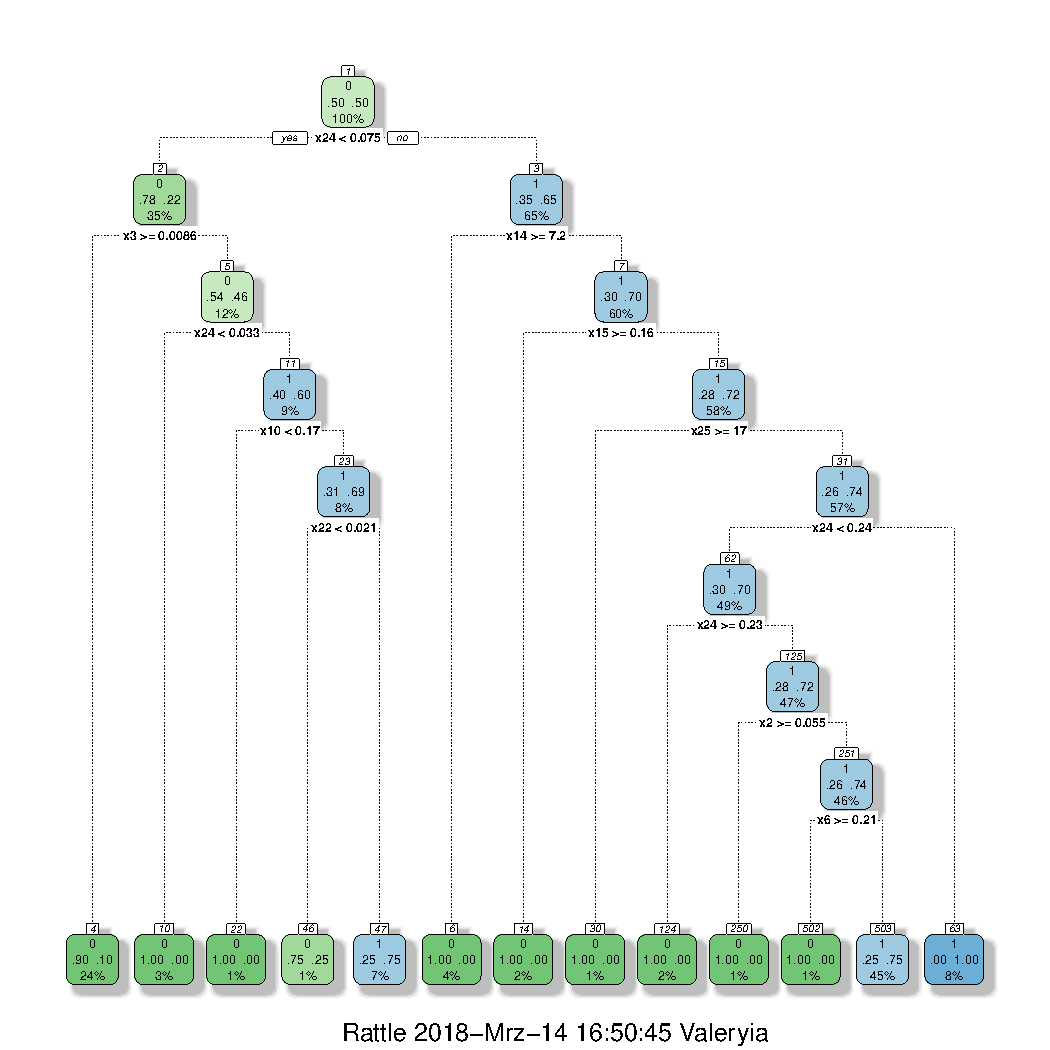
\includegraphics[scale=0.8]{../CART/fancyRpartPlot.pdf}
\end{figure}

fancyRpartPlot() builds more elaborate and clean trees, which can be easily interpreted. Each node box displays the classification, the probability of each class at that specific node and the percentage of observations that arrived at each node (Rickert, 2013). 

Once we have built the model, we are ready to validate it on a separate data set - the test set. We store the results in the object \texttt{mod\_fit} and apply \texttt{predict()} function to calculate the probabilities for further analysis. 

\subsection{Variable Importance}

It might be interesting to acquire information regarding which financial statement variables are most important in predicting the outcome. There are practical reasons for doing so. For example, we want to rank-order financial ratios in regard to their relative importance. This information can provide insights about the most important causes of insolvency, allow a deeper understanding of financial health of the companies and enable investors more effective decision making. If predictor variables were uncorrelated, this would be a simple task. We would rank the predictor variables by their correlation with the response variable. In our case though, the financial ratios variables are correlated (as shown in the chart below), and this complicates the task.
 
We used \texttt{corrplot} package to graphical display a correlation matrix. Positive correlations are displayed in blue and negative correlations in red colour. Colour intensity and the size of the circle are proportional to the correlation coefficients. Every correlation coefficient ranges from 1 to -1, where 1 is a prefect positive correlation, -1 a perfect negative correlation, and 0 indicates no correlation between two features.

\begin{figure}
\caption{Correlation Matrix }
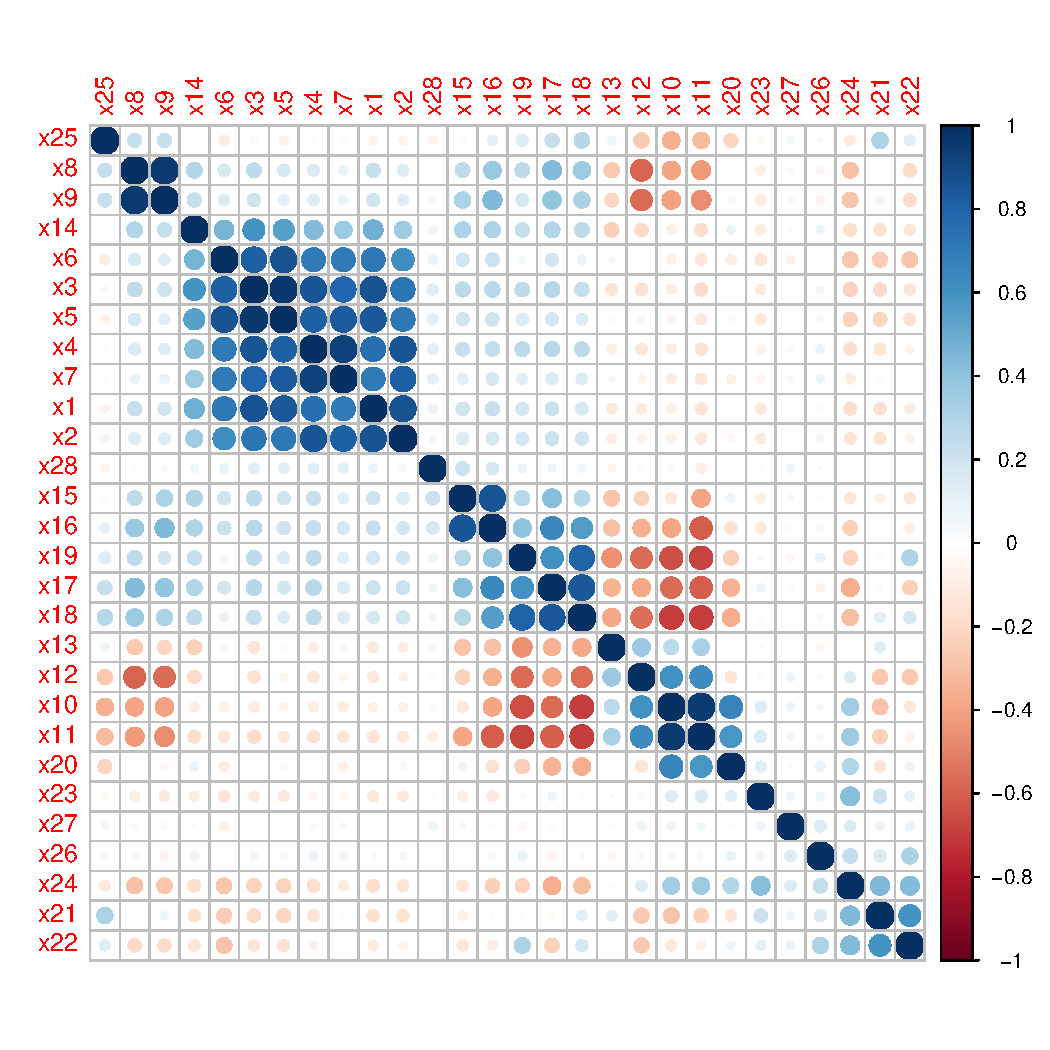
\includegraphics[scale=0.8]{../CART/CorrPlot.pdf}
\end{figure}
%CART/CorrPlot.pdf 

The \texttt{caret}-package includes a command to perform variable importance. \texttt{The varImp()} function calculates important features of almost all models (Kuhn, et al., 2017). We use a call to \texttt{plot} to visualize the results for importance scores generated by the \texttt{varImp()} function. We apply the \texttt{top=10} option to make the chart more readable and select the ten most important variables.

\begin{figure}
\caption{Variable Importance - varImp() function}
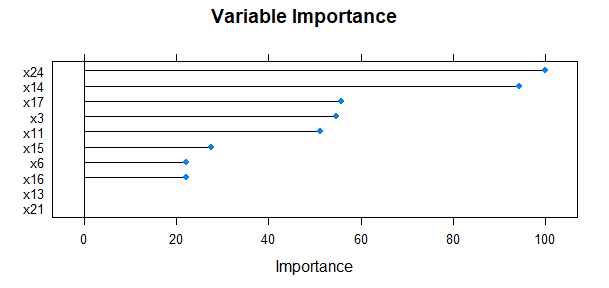
\includegraphics[scale=0.9]{../CART/VarImp_top_10.png}
\end{figure}
%CART/VarImp top 10.png

We can see that the \texttt{varImp function} considers Accounts Payable Turnover (\texttt{x24}) to be the most important feature to predict German default firms, followed by Interest Coverage Ratio Leverage (\texttt{x14}), Quick Ratio \texttt{(x17)}, Operating Income/Total Assets \texttt{(x3)} and Net Indebtedness Leverage \texttt{(x11)}.

All in all, decision trees are an attractive method since they work with many types of data, be it numerical or categorical, without any distributional assumptions and without pre-processing. Furthermore, most of \texttt{R}'s implementations handle missing data. Additionally, this method is robust to redundant and nonlinear data. The algorithm is easy to use, and the graphical output is relatively easy interpretable. On the other hand, decision trees have some shortcomings. They tend to overfit, especially without pruning, because the decision tree can \texttt{memorize} the training set. The model then becomes very specific to the training data and consequently has less ability to classify the unobserved data correctly. Besides, they tend to have a high training variance, which means that samples drawn from the same population can produce trees with different structures and different prediction accuracy. Additionally, a prediction accuracy can be eventually low, compared to other methods. For these reasons a technique called bagging is often used to improve decision tree models. Random Forests are a more specialized approach, which directly combines decision trees with bagging and yields remarkably better results (Zumel \& Mount, 2014). 

\section{Random Forest}

The Random Forest approach often gives an improved predictive accuracy for relatively complex tree models. This ensemble method combines several individual classification trees in the following way: from the original sample several bootstrap samples are drawn, and an unpruned classification tree is fitted to each bootstrap sample. The variable selection for each split in the classification tree is conducted only from a small random subset of predictor variables. From the complete forest the status of the response variable is predicted as an average or majority vote of the predictions of all trees (Maindonald \& Braun, 2010).
\newpage
\lstinputlisting[language=R, firstline=44, lastline=49, firstnumber=44, escapechar=|, caption={|\textbf{\href{https://github.com/thsis/SPL_WS1718/blob/master/Random_Forest/random_forest_modell_fin.R}{random\_forest\_modell\_fin.R}}|}]{../Random_Forest/random_forest_modell_fin.R}
%random_forest_modell_fin line 44-47

We pass several arguments in to the \texttt{randomForest()} function. First of all, since it is a classification problem we define our target variable \texttt{status} as categorical by using \texttt{as.factor()} (Stephens, 2016). In comparison to CART models, trees are grown independently to their maximum extent, limited however by \texttt{nodesize} (minimum number of trees at a node). This parameter implicitly sets the depth of generated trees. Additionally, \texttt{maxnodes} can be used to limit the number of nodes (Maindonald \& Braun, 2010). 

The main tuning parameter is the number \texttt{mtry} of variables that are randomly sampled at each split. By default, the \texttt{randomForest()} function in \texttt{R} draws square root of the total number of variables at each node for classification trees. Essentially, \texttt{mtry} controls the trade-off between the amount of information in each individual tree, and the correlation between trees. Smaller \texttt{mtry} values will grow the trees faster. However, in our case using a larger \texttt{mtry} is better, since we have a large number of variables to choose from, of which only a small fraction is actually useful. By doing so, we are more likely to draw some useful variables at every step of the tree-growing procedure (Zumel \& Mount, 2014).

Further, the \texttt{ntree} argument specifies how many trees we want to grow. By tuning this parameter, the final accuracy of a model might increase up to some point. Also, limiting the number of trees restricts the complexity and computing time (Maindonald \& Braun, 2010). 

Random forests highly increase the prediction accuracy compared to individual classification trees. However, the interpretability of a random forest is not as straightforward as that of an individual classification tree, where the influence of a predictor variable directly corresponds to its position in the tree. Thus, alternative measures for variable importance are required for the interpretation of random forests (Strobl, et al., 2007). 

We can calculate the variable importance by specifying \texttt{importance\=TRUE} in the \texttt{randomForest()} function, and then calling the functions \texttt{importance()} and \texttt{varImpPlot()}. Two measures of importance for each variable are then calculated: \texttt{MeanDecreaseAccuracy} and \texttt{MeanDecreaseGini}. The first measure is a \texttt{leave-one-out} type assessment of variable's contribution to prediction accuracy. Thereby the variable's values are randomly permuted in the out-of-bag samples, and the corresponding decrease in each tree's accuracy is estimated. If the average decrease over all the trees is large, then the variable is considered important - its value makes a big difference in predicting the outcome. If the average decrease is small, then the variable does not make much difference to the outcome. The second measure shows how each variable affects the quality of the tree by representing the decrease in node purity that occurs from splitting on a permuted variable (Maindonald \& Braun, 2010). 

\begin{figure}[H]
\begin{center}
\caption{Variable Importance - \texttt{importance()}-function}
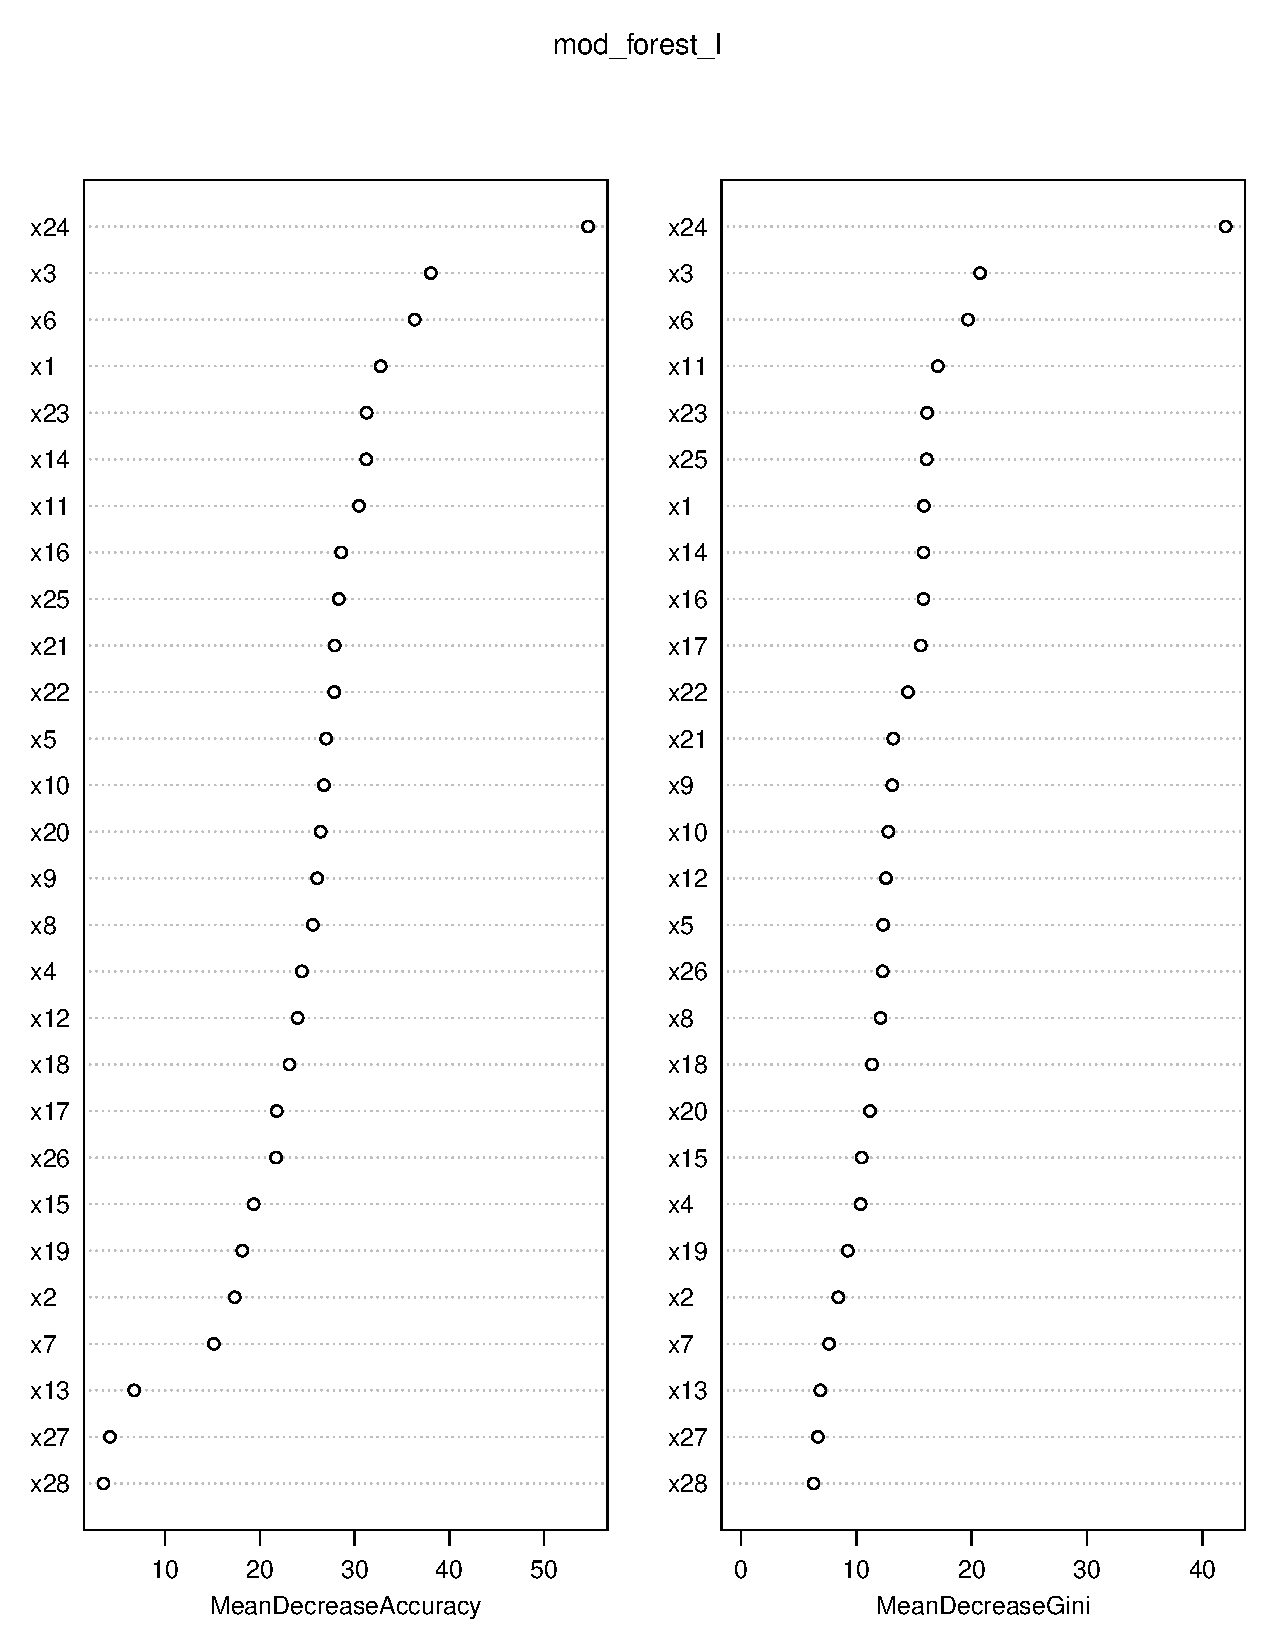
\includegraphics[scale=1, height=8.3cm, width=11cm]{../Random_Forest/Rplot.pdf}
\end{center}
\end{figure}
%Random_Forest/Rplot.pdf

Both measures rate equally the first three and the fifth variables: Accounts Payable Turnover \texttt{x24}, Operating Income/Total Assets \texttt{x3}, EBITDA \texttt{x6} and Account Receivable Turnover Activity \texttt{x23}. Interestingly, this ranking order of \texttt{importance} differs from the results obtained with \texttt{varImp()} function applied for the CART model. Knowing which variables are most important or at least, which variables contribute the most to the structure of the underlying decision trees, can help us with variable reduction. This is useful not only for building smaller, faster trees, but for choosing variables to be used by another modelling algorithm, should that be desired.

The \texttt{random forest} package is robust and very user friendly. However, it is important to note that it has a drawback in that it is invariably biased towards features with many cut points. There is a package \texttt{party} which provides the \texttt{cforest()} command to build a forest of conditional inference trees. The basic construction of each tree is fairly similar to a Random Forest. Hence the decisions are made in slightly different ways, using a statistical test rather than a purity measure. The \texttt{party} package is better than the \texttt{randomForest} package in terms of accuracy, since \texttt{cforest} uses the weighted average of the trees to get the final ensemble. However, it is computationally more expensive (Modi, 2016). In our dataset we do not have features which have many categories and therefore we favour the \texttt{random forest} package to calculate the insolvency predictions. Additionally, it is computationally more efficient.

\section{Evaluation of predictions}

In this section we explain the steps followed in the \texttt{evaluate\_predictions} quantlet. Purpose of this quantlet is to create a function that will take \texttt{labels} (actual solvency status) and \texttt{predictions} about the solvency status of firms and will return the confusion matrix, the ROC curve and the AUC as well as some evaluation metrics like sensitivity, specificity, precision and accuracy.

The confusion matrix, also known as error matrix, is a matrix that illustrates the performance of a classification model on a set of test data with known true values (labels). Each row of the matrix corresponds to a case of a predicted class while each column corresponds to a case of an actual class. It is called confusion matrix because it depicts whether the classifier is confusing the two classes, i.e. if it is wrongly labelling one class as another. It is a special case of a contingency table, with two dimensions ("actual" and "predicted") and two "classes" (solvent and insolvent in our case) in each dimension. The cells of our confusion matrix will present the number of:

\begin{enumerate}
\item True Positives (TP): firms who are correctly predicted to be insolvent (hits).
\item False Positives (FP): solvent firms were wrongly predicted to be insolvent (false alarm or Type I error)
\item False Negatives (FN): insolvent firms were wrongly predicted to be solvent (mass or Type II error)
\item True Negatives (TN): firms were correctly predicted to be solvent (correct rejection) 
\end{enumerate}

These values will then be used to get some important metrics which are described next.

Sensitivity and specificity are assessment metrics of the discriminative power of classification methods (H{\"a}rdle et al., 2012). Sensitivity (also known as the true positive rate) measures the proportion of positives (defaulted firms in our case) that are correctly identified as such (Fawcett, 2006). It is defined as $$TPR=\frac{TP}{TP+FN}.$$ Specificity (or true negative rate) measures the proportion of negatives (solvent firms in our case) that are correctly identified as such (Fawcett, 2006). It is defined as $$TNR=\frac{TN}{TN+FP}.$$ Precision is analogous to the positive predictive value (PPV) and is a measure of exactness (H{\"a}rdle et al., 2012). It is defined as $$PPV=\frac{TP}{TP+FP}.$$ Finally accuracy measures the fraction of correct predictions and is defined as $$ACC = \frac{TP+TN}{TP+TN+FP+FN}.$$

The values of specificity and sensitivity will allow us to plot the ROC curve. The ROC curve (Receiver Operating Characteristic curve) is a graphical plot which depicts the diagnostic ability of a binary classification model for different values of its discrimination threshold. In our case, this threshold refers to the probability value above of which a firm is predicted to be insolvent. It is created by plotting the sensitivity values(y axis) against their corresponding $1-specifity$ values (x axis) as the threshold varies (Fawcett, 2006). The area under the ROC curve (AUC) can be interpreted as the average power of the test on default or non-default corresponding to all discrimination thresholds (H\"ardle et al.(2012)). A larger AUC corresponds to a better classification result. A model with perfect discriminative power will have an AUC value of 1, while a random model without discriminative power will have an AUC value of 0.5, i.e. its ROC curve will be the 45 degree line. Thus, any reasonable rating model is expected to have an AUC value above 0.5, while AUC values close to 1 will indicate models with high diagnostic ability.  

\subsection{Implementation}

\lstinputlisting[language=R, firstline=19, lastline=21, firstnumber=19, escapechar=|, caption={|\textbf{\href{https://github.com/thsis/SPL_WS1718/blob/master/Evaluation/Evaluate_Predictions.fin.R}{Evaluate\_Predictions.fin.R}}|}]{../Evaluation/Evaluate_Predictions.fin.R}

The first function we created in this quantlet is the \texttt{get\_prediction()}-function (lines 19-22). This function takes as inputs the fitted probabilities for insolvency and the threshold above of which a firm would be predicted to be defaulted. Using the \texttt{ifelse()} function in the body of this function, \texttt{get\_prediction()} will return predictions for the solvency status of each firm. We construct then the \texttt{evaluate\_predictions()} function (lines 24-47). Inputs of this function are the actual solvency status of each company (labels), the corresponding predictions about the status and the \texttt{verbose} parameter which is equal to \texttt{FALSE} by default. In the body of the function we create first the previously mentioned confusion matrix which we expect to be a 2x2 matrix. If it is not the case, the test in line 30 will show us a warning message. Then we get the values of TP, TN, FP and FN and we compute the values of sensitivity, specificity, precision and accuracy, which are then saved as a list in \texttt{reports}. The function will also print a data frame with those reports if we change the logical value of \texttt{verbose} to \texttt{TRUE}.

\lstinputlisting[language=R, firstline=24, lastline=45, firstnumber=24, escapechar=|, caption={|\textbf{\href{https://github.com/thsis/SPL_WS1718/blob/master/Evaluation/Evaluate_Predictions.fin.R}{Evaluate\_Predictions.fin.R}}|}]{../Evaluation/Evaluate_Predictions.fin.R}

The final function created in this quantlet is the \texttt{evaluate\_model()} function (lines 49-101), which takes the fitted probabilities for bankrupcy and the actual status (labels) as inputs. At first we create a threshold list in the body of the function with threshold values starting from 0 to 1, which is increased by miniscule steps. Then we apply the \texttt{get\_prediction()} function to this list in order to get a list of predictions for each threshold value which we store as \texttt{pred\_list}. Afterwards we apply the \texttt{evaluate\_predictions()} function to \texttt{pred\_list} and we get a list of reports. We use then the values of sensitivity and specificity from \texttt{reports} in order to compute the ROC curve and the area under it (AUC) (lines 58-70). For calculating the AUC we create the function \texttt{get\_auc()} which takes the values of $1-\texttt{specificities}$ and \texttt{sensitivities} as inputs. This function uses the \href{https://stackoverflow.com/questions/4954507/calculate-the-area-under-a-curve}{trapezoidal method} to approximate the AUC. For each difference in $1-specificities$ there is one rectangle which underestimates the area under curve (corresponding to the "left" value of sensitivities) and one rectangle that overestimates it (corresponding to the "right" value of sensitivities). Therefore the function approximates the AUC by taking the average of the two rectangles. 

\lstinputlisting[language=R, firstline=49, lastline=90, firstnumber=49, escapechar=|, caption={|\textbf{\href{https://github.com/thsis/SPL_WS1718/blob/master/Evaluation/Evaluate_Predictions.fin.R}{Evaluate\_Predictions.fin.R}}|}]{../Evaluation/Evaluate_Predictions.fin.R}


\begin{wrapfigure}[25]{R}{0.3\textwidth}
\caption{ROC Logit}
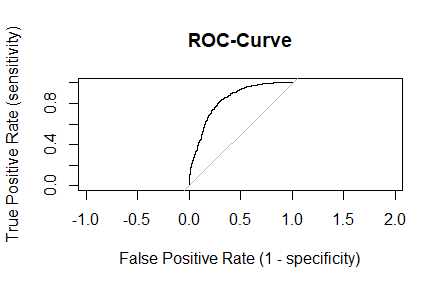
\includegraphics[scale=0.35]{../Evaluation/ROC-Curve_Logit.png}
\caption{ROC CART}
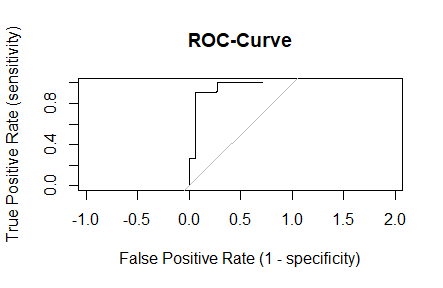
\includegraphics[scale=0.35]{../Evaluation/ROC-Curve_CART.png}
\caption{ROC RF}
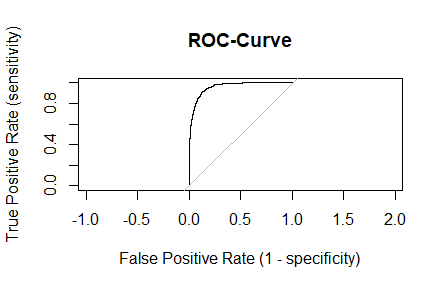
\includegraphics[scale=0.35]{../Evaluation/ROC-Curve_Random-forest.png}
\end{wrapfigure}


We are next interested in finding the values of sensitivities and specificities for which the distance between the ROC curve and the 45-degree line (i.e. the ROC curve of a model with no discriminative power) is maximized. We use the index of these values in order to find the optimal values of sensitivity, specificity and the threshold, which is then used to compute the optimal predictions. These predictions are then used to create the optimal confusion matrix and get the optimal accuracy (lines 73-84). In the final part of the \texttt{evaluate\_model()} function the ROC curve is plotted and the function returns a list with the optimal measures calculated above.


\section{Results and Conclusions}


Logistic regression and decision trees are benchmarking methods in predicting company credit risk. Their modelling techniques are well known for being able to return good probability estimates. Such models can be evaluated in terms of their estimated probabilities. 

Most of the performance measures of a classifier can be read off the entries of confusion matrix. Accuracy measure is largely used to measure a prediction power of a model. Besides, we seek to obtain an idea of more detailed measures such as sensitivity, specificity, and precision. Additionally, we produce the receiver operating characteristic curve (ROC curve) for each method to compare their discriminative power. This metric might provide interesting information for the investors, whose ultimate goal is to reduce losses due to company's bankruptcy. 

The evidence from empirical results consistently shows that a credit risk model based on random forest significantly outperforms CART and Logit approach in modelling the default risk of German firms. Logit model and CART show almost equal accuracy rates, though the values of the area under the curve (AUC), show that the CART classifier do no better than random guessing.

\begin{center}
\begin{table}
\centering
\caption{Classifier performance measure}
\begin{tabular}{cccc}
\hline\hline
Performance measure  &                Logit (\%)   &                  CART(\%)   &     Random forest (\%) \\
\hline
Accuracy Rate        &                 71,6        &                 74,6        &       87,2             \\
Sensitivity          &                 81,6        &                 90,6        &       91,2             \\
Specificity          &                 70,9        &                 73,5        &       87,0             \\
Precision            &                 15,5        &                 18,3        &       31,4             \\
AUC                  &                 82,9        &                 56,1        &       95,8             \\
\hline\hline
\end{tabular}
\end{table}
\end{center}
\newpage
\section{Appendix}

\subsection{Unit Tests}
\subsubsection{LDA}
\begin{wrapfigure}[10]{r}{0.3\textwidth}
\label{iris}
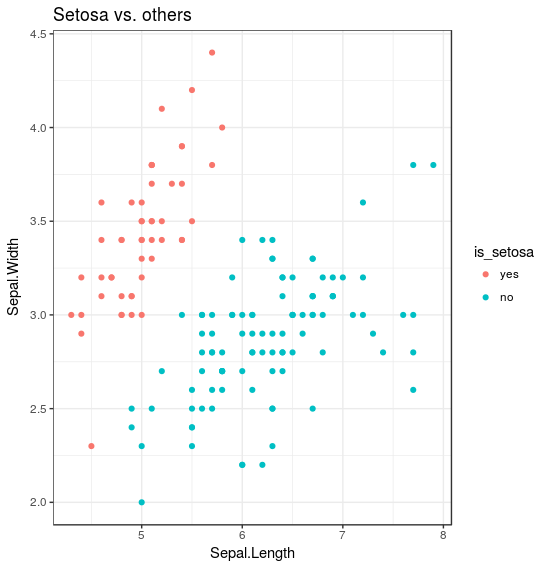
\includegraphics[width=0.2\textwidth, trim={10mm 20mm 30mm 30mm}]{../LDA/iris.png}
\vspace{2mm}
\footnotesize\caption{Setosa species are already linearly separable.}
\end{wrapfigure}

In order to test the \texttt{lda}-function we take a dataset from which we know that it is linearly separable already and see if we can reproduce the results. Since Linear Discriminant Analysis was first proposed by Sir Ronald A. Fisher it is only fitting that we test it on his famous \texttt{iris} dataset. The \texttt{iris} dataset contains measurements of 150 observations for the sepal and petal length and width of three different species of iris flowers. We know that the sepal length and the petal length are sufficient variables to create an obviously visible separation line in figure \ref{iris} which discriminates the Setosa-species almost perfectly from the rest. An exception is one observation of the setosa speces which seems to be an outlier. 

\subsubsection{Expectations}

\begin{wrapfigure}[8]{r}{0.3\textwidth}
\label{irisLDA}
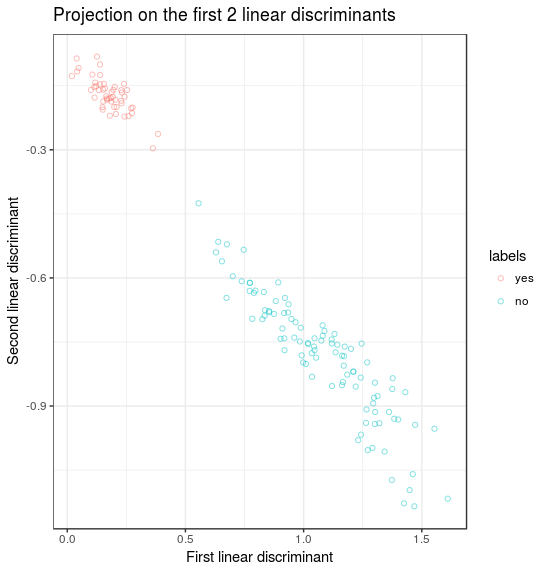
\includegraphics[width=0.2\textwidth, trim={10mm 20mm 30mm 30mm}]{../LDA/irisLDA.png}
\end{wrapfigure}

Should the \texttt{lda}-function work as intended we would expect this result only to become better, i.e. the points being perfectly separable. We first import the \texttt{iris} dataset and transform the Species column in order to fit our binary task, that is we create a dichotomous variable indicating if the particular flower is of the Setosa species or not. We can then directly use the \texttt{lda}-function and plot the first two components against each other.
\subsubsection{Test}
\lstinputlisting[language=R, firstline=26, lastline=27, firstnumber=26, escapechar=|, caption={|\textbf{\href{https://github.com/thsis/SPL_WS1718/blob/master/LDA/lda_tests.R}{lda\_tests.R}}|}]{../LDA/lda_tests.R}

\subsubsection{Result}
As we can see in figure \ref{irisLDA} the two classes are perfectly separable. In fact they would even be separable using only the first linear component.

\subsection{Evaluation}

In order to test the functions used for evaluating the predictions we compare our custom function with the \texttt{auc()} and \texttt{plot.roc()}-functions from the \texttt{pROC}-package. We load the \texttt{Boston} dataset from the \texttt{MASS}-package, which contains data from 506 different census districts of the Boston metropolitan area. 

\subsubsection{Expectations}
For testing purposes we will build a logit-model trying to predict wether the census district is adjacent to the Charles River which is stored in the variable \texttt{chas}. These models are of course nonsense. We will calculate the AUC and plot the ROC-curve once with our home-made function and compare them with the functions from the \texttt{pROC}-package. We would expect that the absolute difference between the two AUC-measures should not be larger than 0.001.

\subsubsection{Test}
\lstinputlisting[language=R, escapechar=|, caption={|\textbf{\href{https://github.com/thsis/SPL_WS1718/blob/master/Evaluation/unit_tests.fin.R}{unit\_tests.fin.R}}|}]{../Evaluation/unit_tests.fin.R}

\subsubsection{Result}
The function passes eleven out of the thirteen tests (84 \%). The plotted ROC-curves were remarkably similar, and the failed tests were caused by especially bad models yielding almost no predictive power. The differences can be mostly attributed to a design decision, we used a step-function, whereas the authors of the \texttt{pROC}-package use a line-plot. However we consider this test a success.
\newpage

\subsection{Code}
\subsubsection{Preparation}
\lstinputlisting[language=R, escapechar=|, caption={|\textbf{\href{https://github.com/thsis/SPL_WS1718/blob/master/Preparation/data.preparation.R}{data.preparation.R}}|}]{../Preparation/data.preparation.R}
\subsubsection{BRM}
\lstinputlisting[language=R, escapechar=|, caption={|\textbf{\href{https://github.com/thsis/SPL_WS1718/blob/master/BRM/utils.R}{utils.R}}|}]{../BRM/utils.R}
\lstinputlisting[language=R, escapechar=|, caption={|\textbf{\href{https://github.com/thsis/SPL_WS1718/blob/master/BRM/logit.R}{logit.R}}|}]{../BRM/logit.R}
\subsubsection{Logit}
\lstinputlisting[language=R, escapechar=|, caption={|\textbf{\href{https://github.com/thsis/SPL_WS1718/blob/master/Logit/logit_model_fin.R}{logit\_model\_fin.R}}|}]{../Logit/logit_model_fin.R}
\subsubsection{CART}
\lstinputlisting[language=R, escapechar=|, caption={|\textbf{\href{https://github.com/thsis/SPL_WS1718/blob/master/CART/cart_modell_fin.R}{cart\_modell\_fin.R}}|}]{../CART/cart_modell_fin.R}
\subsubsection{Random\_Forest}
\lstinputlisting[language=R, escapechar=|, caption={|\textbf{\href{https://github.com/thsis/SPL_WS1718/blob/master/Random_Forest/random_forest_modell_fin.R}{random\_forest\_modell\_fin.R}}|}]{../Random_Forest/random_forest_modell_fin.R}
\subsubsection{LDA}
\lstinputlisting[language=R, escapechar=|, caption={|\textbf{\href{https://github.com/thsis/SPL_WS1718/blob/master/LDA/utils.R}{utils.R}}|}]{../LDA/utils.R}
\lstinputlisting[language=R, escapechar=|, caption={|\textbf{\href{https://github.com/thsis/SPL_WS1718/blob/master/LDA/utils.R}{utils.R}}|}]{../LDA/lda.R}
\subsubsection{Evaluation}
\lstinputlisting[language=R, escapechar=|, caption={|\textbf{\href{https://github.com/thsis/SPL_WS1718/blob/master/Evaluation/Evaluate_Predictions.fin.R}{Evaluate\_Predictions.fin.R}}|}]{../Evaluation/Evaluate_Predictions.fin.R}

\begin{thebibliography}{9}
\bibitem{berk16} 
  Berk, J., DeMarzo, P. (2016), Corporate Finance, 4th edition, Harlow, Pearson Education 
\bibitem{moro11}
  Chen, S., H{\"a}rdle, W.K., Moro, A.R (2011), Modeling default risk with support vector machines,  Quantitative Finance, 11(1), 135-154
\bibitem{duda73}
Duda, R. O., Hart, P. E., Stork, D. G. (1973). Pattern Classification. New York: Wiley-Interscience.
\bibitem {fawcett06}
  Fawcett, T. (2006), An introduction to ROC analysis, Pattern Recognition Letters 27, 861-874
\bibitem{prastyo12} 
  H{\"a}rdle, W.K., Prastyo, D.D., Hafner, C. (2012), Support vector machines with evolutionary model selection for default prediction, SFB 649 Discussion Paper 2012-030
\bibitem{mva03}
H{\"a}rdle, W. K., Simar, L., (2003). Applied Multivariate Statistical Analysis. Heidelberg: Springer-Verlag.
\bibitem{kabacoff11}
Kabacoff, R. I. (2011). R in Action - Data Analysis and graphics with R. Shelter Island, NY 11964: Manning Piblucations Co..
\bibitem{maindonald10}
Maindonald, J. \& Braun, J. W. (2010). Data Analysis and Graphics Using R - an Example-Based Approach. NY: Cambrigde University Press.
\bibitem{miao18} 
  Miao, H., Ramchander, S., Ryan, P., Wang, T. (2018), Default prediction models: The role of forward-looking 
\bibitem{winkel09}
  Winkelmann, R., Boes, S. (2009): \textit{"Analysis of Microdata"}, 2nd edition.
measures of returns and volatility, Journal of Empirical Finance, 46, 146-162
\bibitem{Zhang10} 
  Zhang, J.L., H{\"a}rdle, W.K. (2010). The Bayesian Additive Classification Tree Applied to Credit Risk Modelling. Computational Statistics and Data Analysis, 54: 1197-1205 
\bibitem{Zumel14}
Zumel, N. \& Munt, J. (2014). Practical Data Science with R. Shelter Island, NY 11964: Manning Publications Co..

% Packages
\bibitem{breiman15}
Breiman, L., Cutler, A., Liaw, A. \& Wiener, M. (2015). Package 'randomForest', s.l.: s.n.
\bibitem{kuhn17}
Kuhn, M. et al. (2017). Package 'caret', s.l.: s.n.
\bibitem{milbo16}
Milborrow, S. (2016). Plotting rpart trees with the rpart.plot package, s.l.: s.n.
\bibitem{modi16}
Modi, M. (2016). Different random forest packages in R, s.l.: s.n.
\bibitem{geigen}
Berend, H. (2017). Package 'geigen', s.l.: s.n.
\bibitem{dplyr}
Wickham, H. (2017). Package 'dplyr', s.l.: s.n.

% Online
\bibitem{modiOnl}
Modi, M. (2016). linkedin. [Online] 
Available at: https://www.linkedin.com/pulse/different-random-forest-packages-r-madhur-modi/
\bibitem{rickertOnl}
Rickert, J. (2013). Revolutions. [Online] 
Available at: http://blog.revolutionanalytics.com/2013/06/plotting-classification-and-regression-trees-with-plotrpart.html
\bibitem{robinsonOnl}
Robinson, N. (2018). The Disadvantages of Logistic Regression. [Online] 
Available at: https://classroom.synonym.com/disadvantages-logistic-regression-8574447.html
\bibitem{stephensOnl}
Stephens, T. (2016). Trevor Stephens. [Online] 
Available at: http://trevorstephens.com/kaggle-titanic-tutorial/r-part-5-random-forests/
\bibitem{stroblOnl}
Strobl, C., Boulesteix, A.-L., Zeileis, A. \& Hothorn, T. (2007). BMC Bioinformatics. [Online] 
Available at: https://bmcbioinformatics.biomedcentral.com/articles/10.1186/1471-2105-8-25


\end{thebibliography}
\end{document}